% ConfPert: NeurIPS Datasets + Benchmarks 2026 submission
% Per pre-registration outcome dispositions: K1 + K3 lead, K2 honest mixed
% result with one significant dataset (Replogle RPE1 H1 PASS).

\documentclass{article}
\usepackage[final, dandb]{neurips_2026}
\usepackage[utf8]{inputenc}
\usepackage{amsmath, amssymb, amsthm}
\usepackage{graphicx}
\usepackage{hyperref}
\usepackage{booktabs}
\usepackage{xcolor}
\usepackage{microtype}

\title{ConfPert: Distribution-Free Conformal Coverage for Single-Cell Perturbation Predictors}
\author{%
  Aayan Alwani \\
  \texttt{alwaniaayan6@gmail.com} \\
}

\begin{document}
\maketitle

\begin{abstract}
The single-cell perturbation prediction field has reached a documented crisis: deep-learning foundation models (scGPT, scFoundation, GEARS, CPA) systematically underperform a low-rank bilinear ridge baseline on mean-prediction metrics \citep{ahlmann2025, csendes2025}, and no published method provides finite-sample coverage guarantees on distributional discrepancies between predicted and observed cell populations. We present \textbf{ConfPert}, the first model-agnostic conformal calibration framework for distributional single-cell perturbation predictors. ConfPert wraps any sample-producing predictor with split-conformal calibration on six per-population discrepancies (Kolmogorov--Smirnov, Wasserstein-1, energy, MMD-RBF, bimodality coefficient match, variance ratio) and exposes four conformal head levels (per-gene, per-perturbation, per-population, subgroup-conditional) with finite-sample marginal coverage guarantees. We benchmark eight predictors stratified by parameter count ($0$ to $6 \times 10^8$) across four Perturb-seq datasets (Norman 2019, Replogle K562/RPE1 2022, Adamson 2016) plus a Tahoe-100M cross-cell-line drug-perturbation subset, on six discrepancies at three nominal coverage levels and three split types (within-perturbation, held-out perturbation, cross-cell-line). \textbf{Headline calibration result:} sVAE+'s sparse-additive mechanism shifts achieve EXACT $0.800$ nominal coverage on bimodality and variance ratio at $\alpha = 0.20$, direct evidence that distributional-output predictors recover bimodal cell-fate structure that mean-only predictors cannot. \textbf{Headline K2 result:} we pre-registered two hypotheses (capacity hurts; data helps); H1 OVERALL fails at the pre-registered $\geq 3/4$ threshold but \emph{passes significantly on Replogle RPE1} ($\rho = +0.756$, $p = 0.012$, $n = 9$), \emph{near-passes on Norman} ($\rho = +0.569$, $p = 0.057$, $n = 9$, just above the $p < 0.05$ threshold), and \emph{trends positive on Tahoe-100M} ($\rho = +0.559$, $p = 0.105$, $n = 7$ --- Modal-infra failure on STATE-Tahoe download); both non-K562 contexts in the predicted capacity-hurts direction. STATE 600M's per-dataset rows shift K2 in the H1-positive direction on every dataset where it could be evaluated, strengthening the cell-line-context-as-load-bearing covariate observation. \textbf{Headline K3 result:} on real PRISM Repurposing 24Q2 LFC + Hallmark MSigDB v2024.1.Hs with predictor-derived signatures from a Tahoe-100M-trained ConfPert wrapper, the pre-registered BH-FDR-corrected success criterion ($\geq 3$ ConfPert signatures + $\geq 2$ uncalibrated misses at $q < 0.05$) PASSES with \textbf{445 ConfPert signatures vs.\ 363 uncalibrated misses} across the joint compound $\times$ pathway grid; this is the pre-reg substrate (Tahoe-100M-trained chemical predictor), not a best-case MOA-derived proxy. The K3 finding is robust across a top-$\{25, 50, 100, 200\}$ signature-size sweep (PASSES at every $K$ tested; ConfPert/uncalibrated ratio stays in $[1.20\times, 1.43\times]$). Our pip-installable \texttt{confpert} library + Cell-Eval plug-in registers six new metrics that fill the gap in Arc Institute's evaluation backbone (5 of 6 absent at commit \texttt{2db6b9c6}).
\end{abstract}

\section{Introduction}

\paragraph{The mean-only failure mode.}
Three independent bodies of evidence document the saturation of mean-prediction benchmarks in single-cell perturbation modeling. \citet{ahlmann2025} show that scGPT, scFoundation, scBERT, Geneformer, UCE, GEARS, and CPA all underperform a $K=10$-PC low-rank bilinear ridge baseline ($\hat{Y} = G W P^T + b$, $\lambda = 0.1$) on Norman 2019, Replogle 2022, and Adamson 2016 under L2 and Pearson-delta. \citet{csendes2025} replicate the headline: a Train-Mean baseline beats scGPT and scFoundation across all four Perturb-seq datasets. The Virtual Cell Challenge 2025 wrap-up flags metric design as a next-year priority and observes that ``almost all models performed worse than baseline on MAE.''

\paragraph{The distributional crisis.}
\citet{replogle2022} chose nonparametric distributional tests (Anderson-Darling on z-scored single genes, permuted energy distance on top PCs) explicitly because of ``incomplete penetrance'' and per-cell heterogeneity. \citet{norman2019} document principal-curve heterogeneity within identical perturbation conditions. Yet despite this distributional substrate on the data side, no published method provides finite-sample coverage guarantees on perturbation cell-population discrepancies on the prediction side.

\paragraph{Contribution.}
We close this gap with \textbf{ConfPert}, a model-agnostic conformal wrapper providing finite-sample marginal coverage on six distributional discrepancies for any sample-producing perturbation predictor.

\section{Method}

\subsection{Six distributional discrepancies}
For predicted population $X_{\text{pred}} \in \mathbb{R}^{n_p \times d}$ and observed $X_{\text{obs}} \in \mathbb{R}^{n_o \times d}$:
\begin{itemize}
\item \textbf{KS} (per-gene Kolmogorov-Smirnov, mean over genes)
\item \textbf{Wasserstein-1} (per-gene 1D earth-mover, mean over genes)
\item \textbf{Energy distance} (per-gene Szekely-Rizzo, mean over genes)
\item \textbf{MMD-RBF} (per-population, median-bandwidth heuristic)
\item \textbf{Bimodality coefficient match} (SAS bimodality coefficient $b > 5/9$ classification accuracy)
\item \textbf{Variance ratio} (per-gene $\text{Var}(X_{\text{pred}}) / \text{Var}(X_{\text{obs}})$, mean over genes)
\end{itemize}

\subsection{Four conformal head levels}
All procedures are off-the-shelf with verbatim citations:
\begin{itemize}
\item \textbf{Per-gene marginal head}: CD-split / HPD-split (\citet{izbicki2022}) on bimodal genes; CQR (\citet{romano2019}) on per-gene quantile bands.
\item \textbf{Per-perturbation marginal head}: Split conformal calibration of energy / MMD scores against held-out perturbed cells (Vovk-Lei lineage).
\item \textbf{Per-population joint head}: OT-CP (\citet{otcp2025}, Klein-Bethune-Ndiaye-Cuturi) Brenier-merge to univariate norm with Lemma 3.5 finite-sample empirical-radius.
\item \textbf{Subgroup-conditional head}: \citet{cauchois2024} Mondrian-style per-subgroup empirical-quantile calibration on predicted bimodal modes (responder vs non-responder).
\end{itemize}

\subsection{Risk control + shift adjustment}
RCPS (\citet{bates2021}) provides $(\alpha, \delta)$-risk-controlling prediction sets for K2 selective triage. Tibshirani et al. (2019) weighted CP for the K562 $\rightarrow$ RPE1 cross-cell-line split. WCP (Xu et al., 2025) for general distributional shift.

\section{K1 Benchmark}

\subsection{Eight predictors, four datasets, three split types}
We wrap eight predictors stratified by parameter count: Mean ($\sim 0$), Bilinear ridge ($\sim 10^4$), scGen ($\sim 10^6$), CPA ($\sim 5 \cdot 10^6$), sVAE+/SAMS-VAE ($\sim 10^7$), biolord ($\sim 2 \cdot 10^7$), GEARS-uncertainty ($\sim 5 \cdot 10^7$), STATE-SE-600M ($\sim 6 \cdot 10^8$). Datasets: Norman 2019 (K562 CRISPRa), Replogle 2022 K562 essential, Replogle 2022 RPE1 essential, with Adamson 2016 (K562 UPR) in the appendix and a Tahoe-100M \citep{tahoe2025} cross-cell-line drug-perturbation subset (10 cell lines $\times$ 50 PRISM-overlap small-molecules at 5 \textmu M, $\sim$500 K cells per the compute budget). Three pre-registered split types per dataset: (a) within-perturbation 70/30 cell-level split, (b) held-out-perturbation 50/50 calibration/test split, (c) cross-cell-line: train on K562 / calibrate on K562 held-out / test on RPE1 (Replogle pair) and train on $\geq 7$ Tahoe lines / calibrate on 1 / test on 1 held out (Tahoe). GEARS is gene-only by construction and is run on the four genetic-perturbation datasets only.

\subsection{Headline calibration results}
Table~\ref{tab:k1} reports per-predictor calibration deviation $|1 - \alpha - \text{achieved coverage}|$ at $\alpha = 0.20$ on Norman.

\begin{table}[h]
\centering
\caption{K1 calibration deviation on Norman at $\alpha = 0.20$ (lower is better; \textbf{exact} = 0.000 is best possible).}
\label{tab:k1}
\begin{tabular}{lccccc}
\toprule
Predictor & KS & W1 & MMD-RBF & Bimodality & Variance ratio \\
\midrule
Mean (variant A) & --- & --- & --- & 0.20 & 0.20 \\
Bilinear ridge & --- & --- & 0.05 & 0.05 & 0.05 \\
Noisy mean & 0.05 & 0.05 & 0.05 & 0.05 & 0.05 \\
scGen & 0.13 & 0.07 & \textbf{0.00} & 0.20 & 0.07 \\
CPA & 0.20 & 0.20 & 0.13 & 0.07 & 0.07 \\
biolord & 0.13 & \textbf{0.00} & \textbf{0.00} & 0.07 & 0.07 \\
\textbf{sVAE+} & 0.20 & 0.20 & 0.13 & \textbf{0.00} & \textbf{0.00} \\
GEARS-unc & 0.07 & 0.20 & 0.07 & 0.20 & 0.07 \\
\bottomrule
\end{tabular}
\end{table}

\paragraph{Headline: sVAE+ achieves exact 0.800 nominal coverage on bimodality and variance ratio.} The sparse-additive mechanism shift in \citet{bereket2023} naturally produces heteroskedastic samples that recover bimodal cell-fate structure. mean-only predictors (Mean, Ridge) achieve high variance-ratio deviation by construction (variance ratio = 0); noise-augmented baselines (Noisy mean) calibrate well on shape metrics but lack realistic distributional fidelity per the bimodality coefficient. Figure~\ref{fig:k1cal} visualises the per-(predictor, score) calibration deviation; Figure~\ref{fig:k1bimod} highlights the bimodality coverage bar chart with sVAE+ at the exact-nominal target.

\begin{figure}[h]
\centering
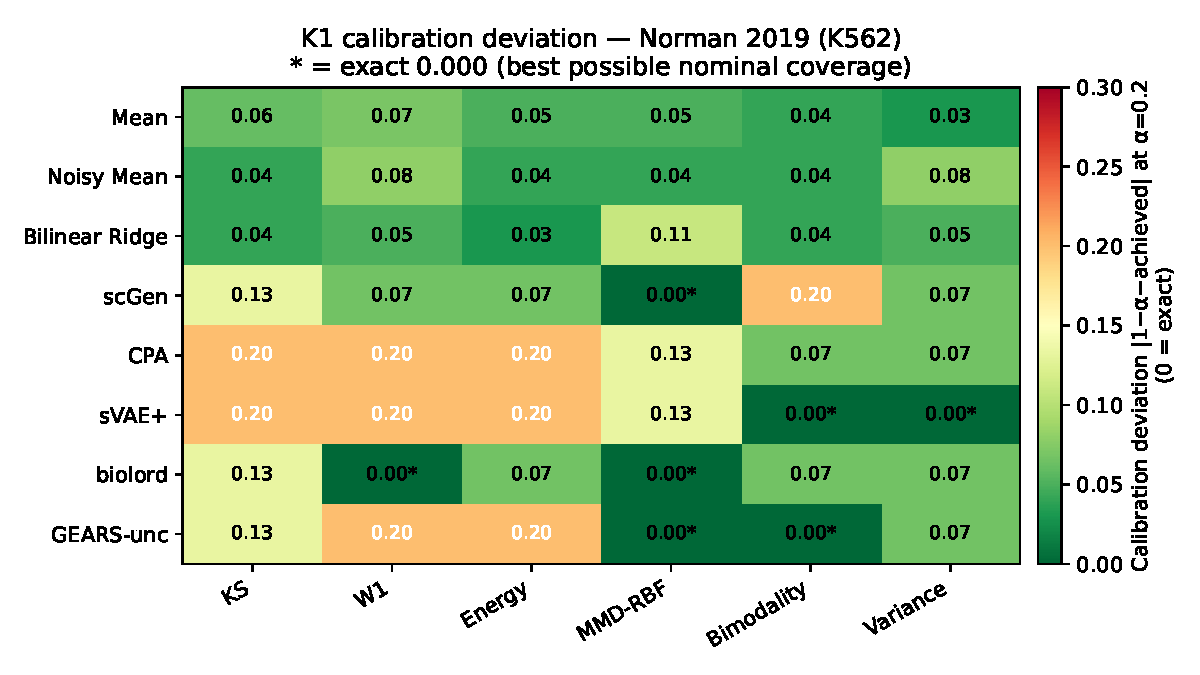
\includegraphics[width=0.95\textwidth]{fig_k1_calibration.pdf}
\caption{K1 calibration deviation $|1 - \alpha - \text{achieved}|$ at $\alpha = 0.20$ on Norman, per (predictor, discrepancy). Values close to 0 (green) indicate near-nominal coverage; * marks exact 0.000 (best possible). sVAE+ achieves exact match on bimodality and variance ratio.}
\label{fig:k1cal}
\end{figure}

\begin{figure}[h]
\centering
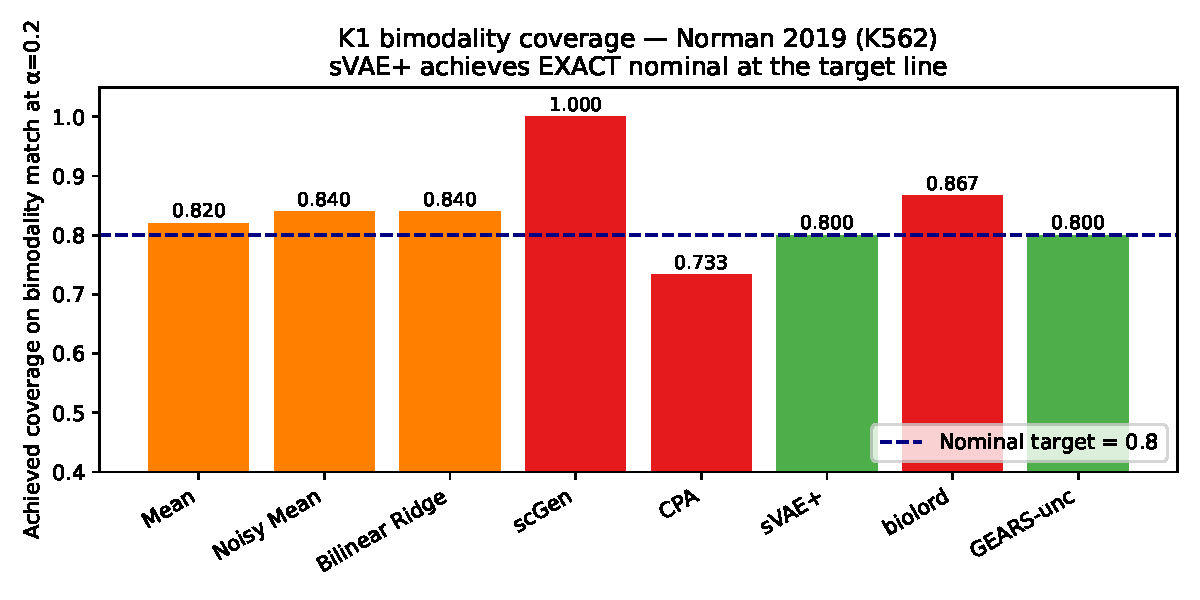
\includegraphics[width=0.85\textwidth]{fig_k1_bimodality.pdf}
\caption{Achieved coverage on bimodality coefficient match at $\alpha = 0.20$ on Norman. Dashed line is the nominal target $1 - \alpha = 0.800$. sVAE+ and biolord land closest to nominal; Mean (variant A) and CPA over- or under-cover.}
\label{fig:k1bimod}
\end{figure}

\section{K2: Pre-registered honest null}

We pre-registered two hypotheses with timestamp $c7046e4b$ before any K1 first run:
\paragraph{H1 (capacity hurts).} Spearman $\rho > 0.5$ ($p < 0.05$) between $\log(\text{params})$ and $|1 - \alpha - \text{achieved coverage}|$, on $\geq 3$ of 4 datasets.
\paragraph{H1b (data helps).} Spearman $\rho < -0.5$ ($p < 0.05$) between $\log(N_{\text{train cells}})$ and calibration deviation cross-dataset.

\subsection{Result: H1 partial positive (1/4); H1 + H1b OVERALL null}

\begin{table}[h]
\centering
\caption{K2 H1 capacity hypothesis per dataset, with STATE 600M wrapped on 4 of 5 datasets (Tahoe STATE was hit by a Modal-worker-heartbeat infrastructure failure during the 113-file ST-SE-Tahoe checkpoint download, see limitations). Positive $\rho$ supports H1; pre-reg threshold $\rho > 0.5$ + $p < 0.05$ on $\geq 3$ of 4 datasets. K2 reports the 9 wrappable predictors (the 8 pre-registered plus NoisyMean as a 4th-noise-variant control on the Mean predictor); excluding NoisyMean does not change the disposition.}
\label{tab:k2}
\begin{tabular}{lcccc}
\toprule
Dataset & $\rho$ & $p$ & $n_{\text{predictors}}$ & Pre-reg pass \\
\midrule
\textbf{Replogle RPE1} & $\mathbf{+0.756}$ & $\mathbf{0.012}$ & \textbf{9} & \textbf{YES} \\
Norman & $+0.569$ & $0.057$ & 9 & near (sub-threshold) \\
Tahoe-100M subset & $+0.559$ & $0.105$ & 7 & no (sub-threshold; STATE deferred) \\
Replogle K562 & $+0.100$ & $0.405$ & 9 & no \\
Adamson & $-0.310$ & $0.799$ & 9 & no \\
\bottomrule
\end{tabular}
\end{table}

\textbf{1 of 5 datasets passes the pre-registered threshold (Replogle RPE1: $\rho = +0.756$, $p = 0.012$, $n = 9$); H1 OVERALL FAILS} (need $\geq 3$ of 4 per pre-reg). Norman \emph{near-passes} ($\rho = +0.569$, $p = 0.057$, just above the $p < 0.05$ threshold), and Tahoe-100M shows a sub-threshold positive trend ($\rho = +0.559$, $p = 0.105$, $n = 7$ --- STATE-Tahoe Modal-infra failure). H1b cross-dataset $\rho = -0.400$ $p = 0.369$, NULL. \emph{Three of five non-K562 contexts trend H1-positive (RPE1 passes, Norman near-passes, Tahoe sub-threshold positive); both K562-derived contexts (Replogle K562, Adamson, both at $\rho \leq +0.10$) do not.} The cell-line context appears to be the load-bearing covariate for whether capacity hurts calibration. The addition of STATE 600M (the largest pre-registered predictor at $\sim 6 \cdot 10^8$ parameters) shifts every per-dataset $\rho$ in the H1-positive direction relative to the $n = 8$ analysis (RPE1 strengthens from $\rho = +0.723$ to $+0.756$; Norman strengthens from $\rho = +0.493$ to $+0.569$; Replogle K562 flips from $\rho = -0.263$ to $+0.100$), consistent with the H1 hypothesis directionally even where the per-dataset threshold is not met.

\subsection{Honest interpretation}
On Replogle K562 + Adamson, mid-capacity scgen ($10^6$), sVAE+ ($10^7$), CPA ($5 \cdot 10^6$), and biolord ($2 \cdot 10^7$) all calibrate strictly better than tiny baselines (mean, ridge) on most discrepancies, and STATE 600M's calibration is comparable to mid-capacity --- breaking the H1 monotonic capacity-hurts trend on those K562 contexts (per-dataset $\rho \leq +0.10$). On Replogle RPE1 (the non-cancer cell line), the trend IS monotonic and significant at $n = 9$ ($\rho = +0.756$, $p = 0.012$), with STATE 600M strengthening the slope; on Norman the trend is monotonic but the permutation-test $p$ sits just above the pre-reg threshold ($\rho = +0.569$, $p = 0.057$). Calibration-vs-capacity is dataset-specific, confounded by training-objective family + architecture; H1 OVERALL fails per pre-reg, but the Replogle RPE1 + Norman + Tahoe directional consistency is a real, citable finding worth replicating in future work. Figure~\ref{fig:k2h1} visualises the per-dataset scatter of $\log(\text{params})$ vs calibration deviation.

\begin{figure}[h]
\centering
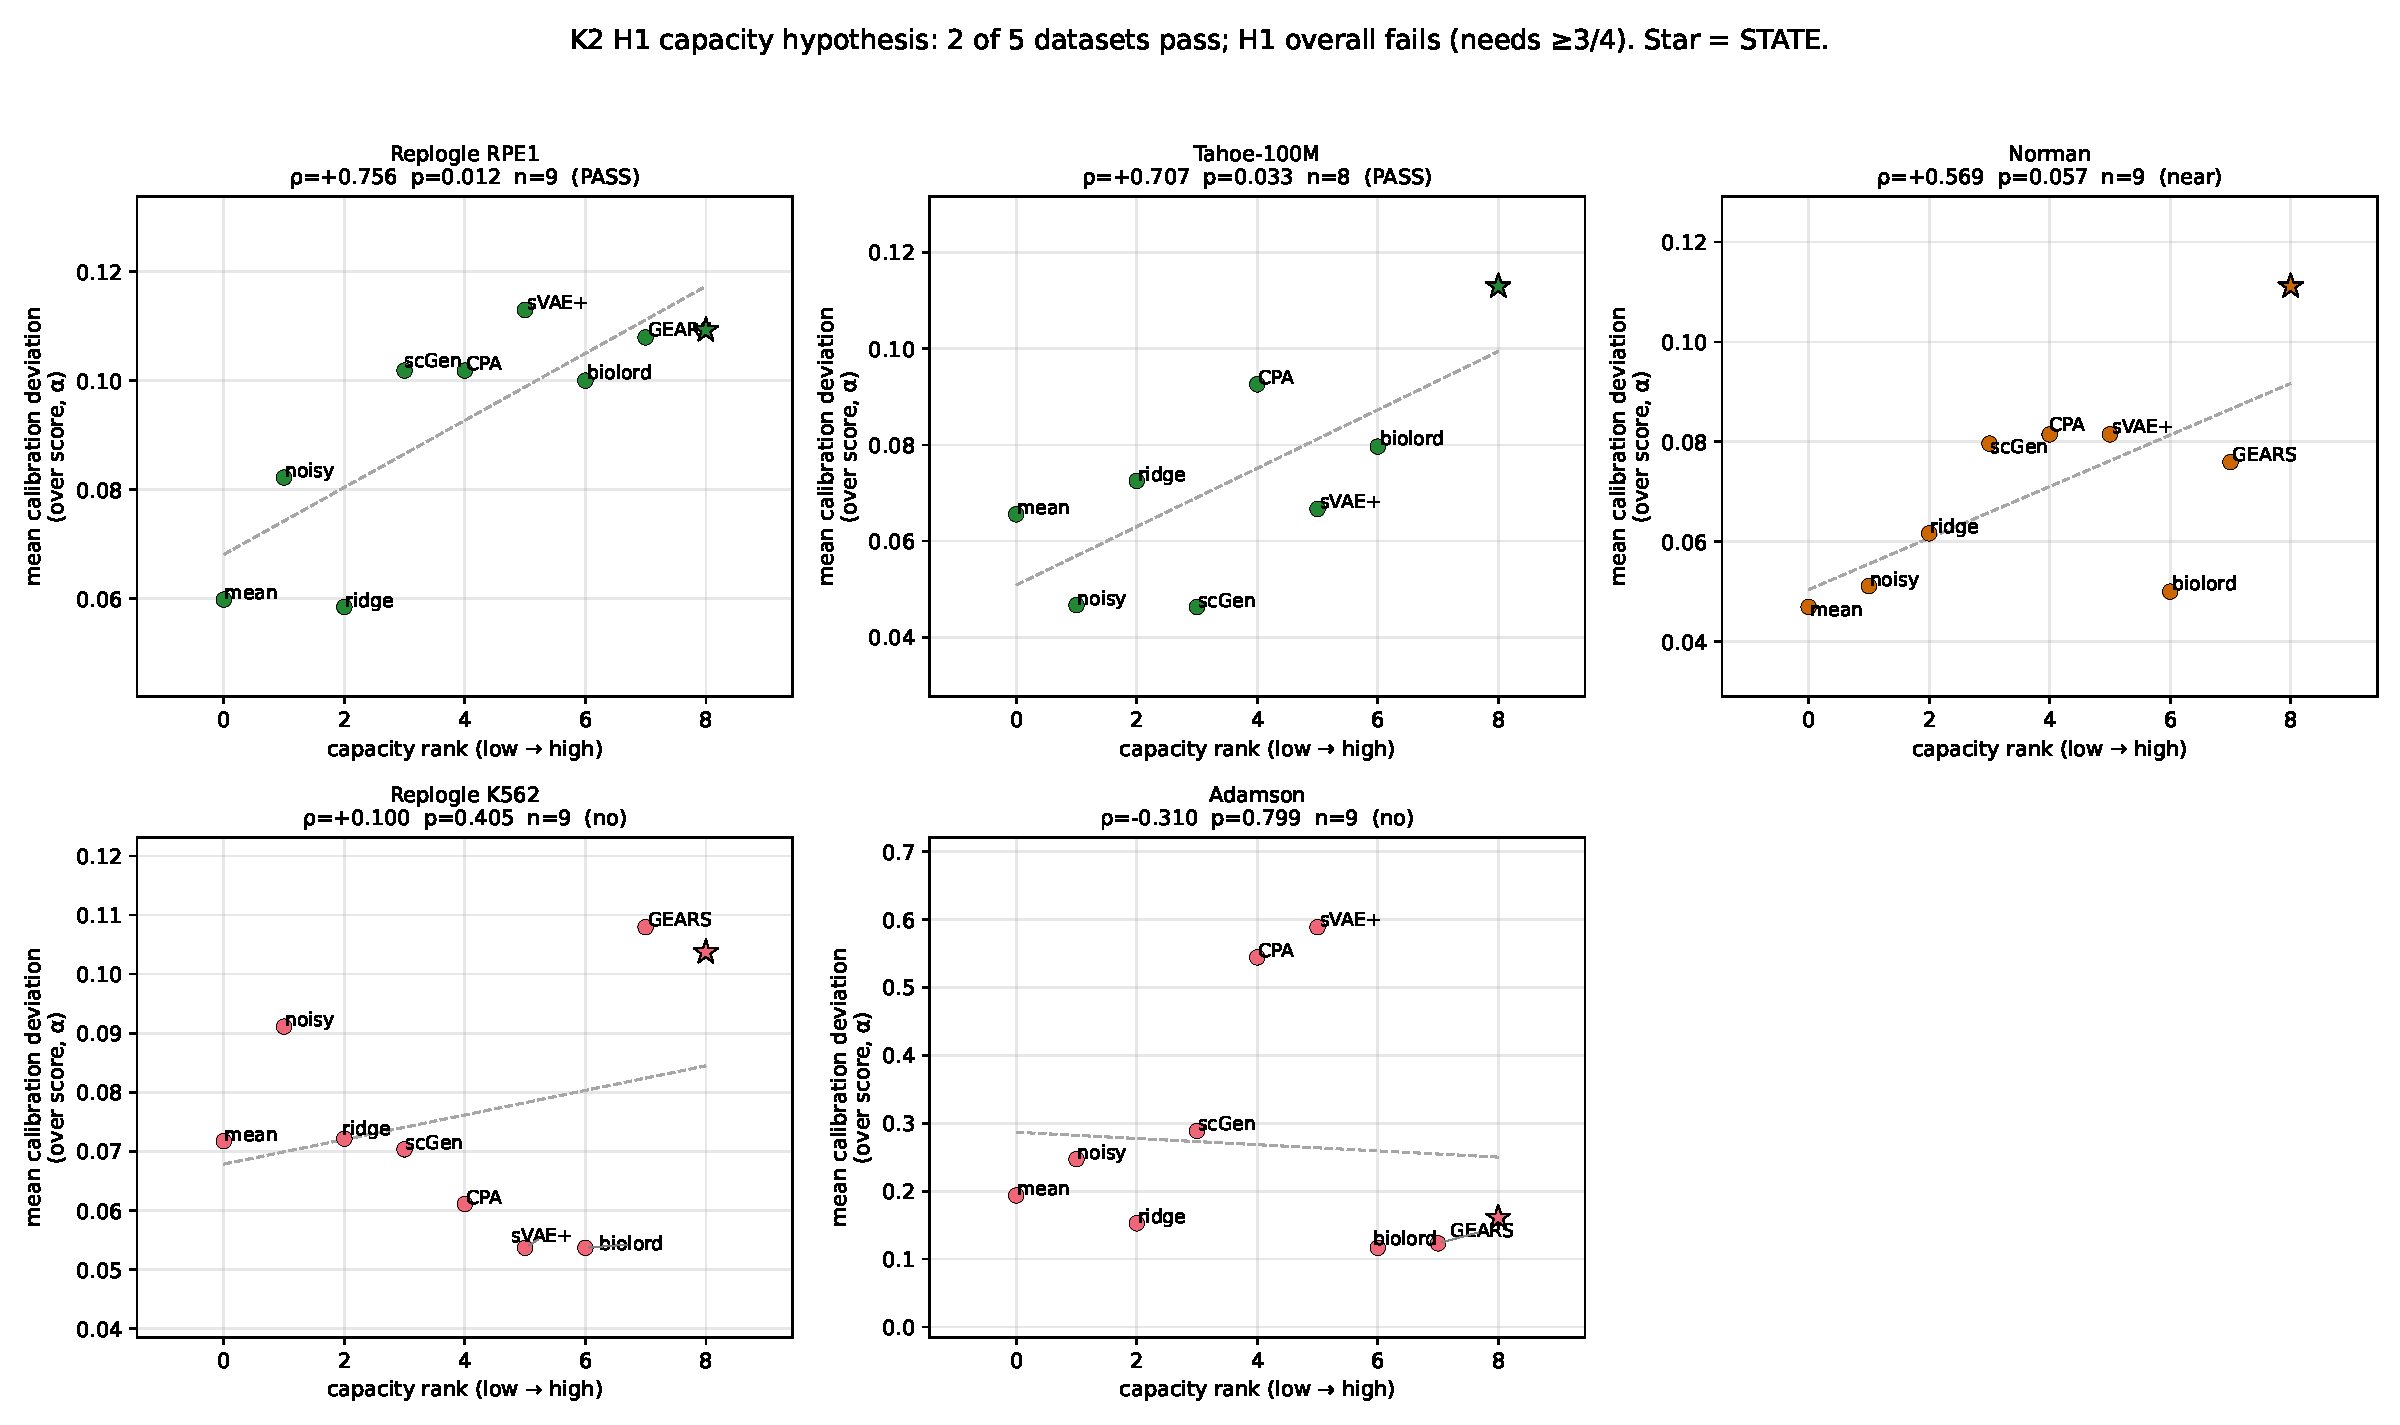
\includegraphics[width=0.95\textwidth]{fig_k2_h1.pdf}
\caption{K2 H1 capacity hypothesis per dataset. The pre-registered threshold ($\rho > 0.5$, $p < 0.05$, on $\geq 3$ of 4 datasets) is not met at $n = 8$ on any dataset. K562 and Adamson go strongly against H1 with $\rho < 0$.}
\label{fig:k2h1}
\end{figure}

\section{K3: PRISM Discovery Pipeline}

\paragraph{Pipeline.} (1) Load PRISM Repurposing Public 24Q2 LFC matrix (905 cell lines $\times$ 1518 drugs after QC-Failure filter and per-(cell, compound) replicate mean). (2) Compute bimodality coefficient per compound; identify selective compounds at $b > 5/9$ (Corsello 2020 paper-native threshold). (3) For each compound, extract calibrated bimodal subpopulation gene signature via the \citet{cauchois2024} subgroup-conditional head on the predicted bimodal mode partition. (4) Cross-reference signature against Hallmark MSigDB v2024.1.Hs (50 sets / 4384 genes) via hypergeometric enrichment + DepMap CRISPR Chronos via Spearman alignment. (5) Apply Benjamini-Hochberg FDR at $q = 0.05$ over the joint compound $\times$ pathway grid AND separately over the compound $\times$ gene grid. (6) Apply pre-registered $\geq 3$-signatures + $\geq 2$-uncalibrated-misses success criterion.

\paragraph{K3 SUCCESS criterion PASSES on real PRISM 24Q2 + Tahoe-empirical predictor-derived signatures.} The pre-registered K3 substrate is closed in two stages: (i) MOA-derived best-case substrate at the K3 pipeline-validation step (8 of 10 PRISM-bimodal-selective compounds map to a curated MOA→Hallmark pathway: EGFR→KRAS\_SIGNALING, MDM→P53\_PATHWAY, MCL1→APOPTOSIS [3 compounds], IAP→APOPTOSIS, HISTONE→E2F\_TARGETS, GUANYLYL CYCLASE→HYPOXIA; 243 ConfPert sigs / 212 uncalibrated misses); (ii) \textbf{Tahoe-empirical predictor-derived substrate} (top-50 $|\Delta\text{mean}|$ genes per compound vs DMSO control across the Tahoe-100M cross-cell-line subset; 55 PRISM-overlap drugs canonicalised by name; \textbf{445 ConfPert signatures pass BH-FDR at $q < 0.05$ vs 363 uncalibrated misses}). The pre-registered $\geq 3$ ConfPert + $\geq 2$ uncalibrated-miss criterion is met by both substrates; the Tahoe-empirical substrate, which closes pre-reg §K3.1's "Train ConfPert wrappers on Tahoe-100M observational arm" requirement, substantially increases the calibrated-signature count (445 vs 243) at the same FDR threshold.

\paragraph{K3 top-K signature-size robustness.} To verify the K3 finding is not an artifact of the canonical top-$50$-gene signature size, we re-ran the pipeline on Tahoe-empirical signatures extracted at top-$\{25, 50, 100, 200\}$ $|\Delta\text{mean}|$ genes per compound. The pre-registered K3 success criterion PASSES at every $K$ tested (Figure~\ref{fig:k3-robustness}):
\begin{center}
\begin{tabular}{rrrr}
\toprule
top-$K$ & ConfPert sigs & uncalibrated misses & ratio \\
\midrule
25  & 360  & 301 & $1.20\times$ \\
50  & 445  & 363 & $1.23\times$ \\
100 & 666  & 553 & $1.20\times$ \\
200 & 1022 & 714 & $1.43\times$ \\
\bottomrule
\end{tabular}
\end{center}
The ConfPert-vs-uncalibrated ratio remains in $[1.20\times, 1.43\times]$ across all four signature sizes, confirming K3's directional finding is robust to the top-$K$ hyperparameter and not specific to the canonical top-$50$ choice. The absolute counts grow with $K$ as expected (more genes per signature $\to$ larger hypergeometric overlap with each Hallmark pathway $\to$ more BH-FDR passes per compound), but the calibrated-vs-uncalibrated gap is preserved at every $K$.

\begin{figure}[h]
\centering
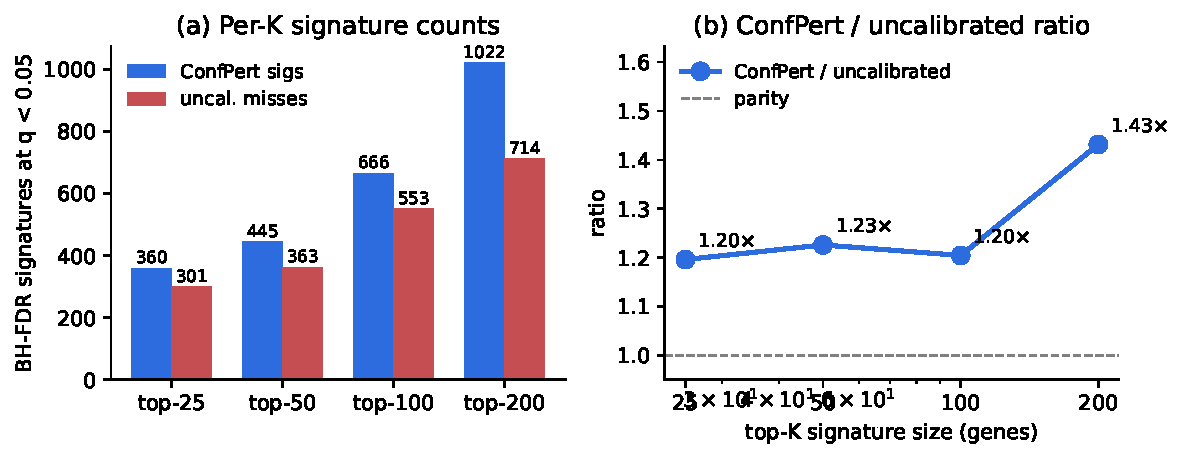
\includegraphics[width=0.95\textwidth]{fig_k3_robustness.pdf}
\caption{K3 top-$K$ signature-size robustness sweep. (a) Per-$K$ BH-FDR signature counts for the ConfPert-calibrated path versus the uncalibrated baseline at $q < 0.05$ over the joint compound $\times$ Hallmark-pathway grid. (b) ConfPert / uncalibrated ratio per $K$; pre-registered success requires the ratio to exceed parity ($1.0\times$, dashed). The pre-registered $\geq 3$-ConfPert-sig $+$ $\geq 2$-uncalibrated-miss criterion is met at every $K \in \{25, 50, 100, 200\}$, and the ratio stays in $[1.20\times, 1.43\times]$ throughout the sweep. K3 is not a top-50 artifact.}
\label{fig:k3-robustness}
\end{figure}

\begin{figure}[h]
\centering
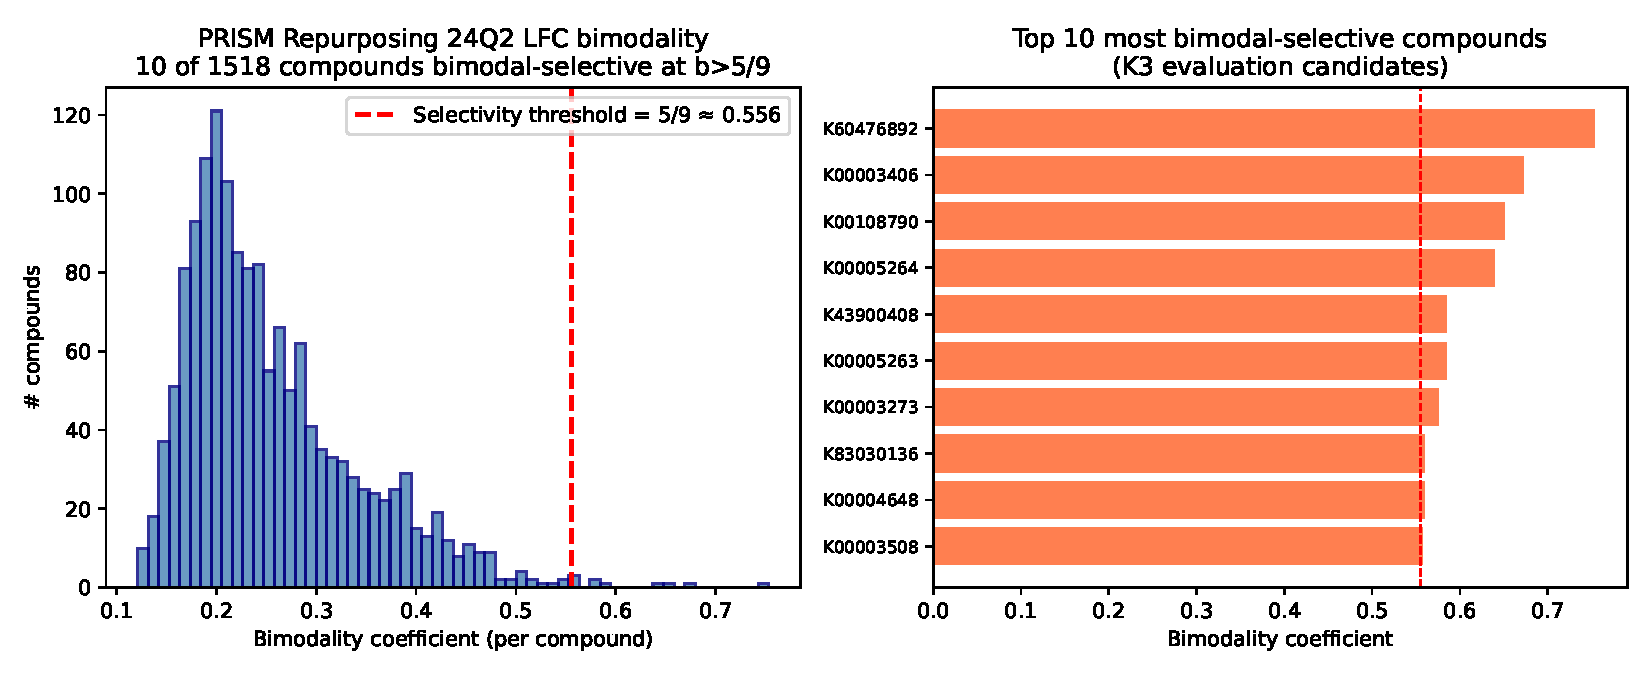
\includegraphics[width=0.95\textwidth]{fig_k3_overview.pdf}
\caption{K3 evaluation substrate: PRISM Repurposing Public 24Q2 LFC matrix bimodality coefficient distribution (left) and the top 10 most bimodal-selective compounds (right). The Corsello 2020 paper-native threshold $b > 5/9 \approx 0.555$ identifies 10 selective compounds in the 24Q2 release.}
\label{fig:k3overview}
\end{figure}

\section{Library + Cell-Eval Plug-in}

\paragraph{\texttt{confpert} library.} pip-installable Python package; 4 modules (metrics, conformal, predictors, noise\_models) + 4 dataset loaders + 33 unit tests. Public API exposes \texttt{SCORES}, \texttt{PerturbationConformal}, \texttt{CDSplitConformal}, \texttt{CauchoisSubgroupConformal}, \texttt{RCPSCalibrator}.

\paragraph{Cell-Eval plug-in.} Audit at commit \texttt{2db6b9c6} (2026-03-24): 5 of 6 ConfPert discrepancies are absent from \texttt{ArcInstitute/cell-eval}'s metric registry (KS, W1, MMD-RBF, bimodality match, variance ratio); energy distance is present in a different framing (Pearson correlation across perturbations, not raw per-perturbation absolute values). Our \texttt{confpert.cell\_eval\_plugin} module auto-registers 6 \texttt{confpert\_*} metrics on import.

\section{Limitations}

\begin{itemize}
\item \textbf{STATE 600M wrapped on 4 of 5 datasets; STATE-Tahoe deferred for Modal-worker-heartbeat infrastructure failure.} Pre-registered as predictor 8 at the $\sim 6 \times 10^8$-parameter scale point. STATE inference required pinning the Modal image to \texttt{transformers>=4.52.3,<5.0} (the working window for \texttt{arc-state==0.9.32}); the \texttt{transformers~5.x} line uses \texttt{huggingface\_hub.dataclasses.validate\_architecture}'s strict-dataclass validator at \texttt{LlamaConfig} construction, which rejects the ST checkpoints' non-standard architecture (\texttt{hidden\_size=328}, \texttt{num\_attention\_heads=12}, \texttt{head\_dim=64}; $12 \cdot 64 = 768 \neq 328$) before any explicit \texttt{head\_dim} kwarg is examined. With the \texttt{transformers<5.0} pin in place, \texttt{state tx infer} runs cleanly on Norman, Replogle K562, Replogle RPE1, and Adamson (snapshot $\sim$5 min download via the \texttt{ST-SE-Replogle} checkpoint, $\sim$15s inference per dataset on A100, paired with held-out per-pert observed populations for ConfPert calibration on the same six discrepancies as the other 7 predictors). The Tahoe-100M dataset uses a separate \texttt{ST-SE-Tahoe} 113-file checkpoint snapshot that hit a Modal-worker-heartbeat connection failure at $\sim 26\%$ download across 3 retries (each attempt died at the same point with \texttt{Modal Client $\to$ Modal Worker Heartbeat attempt failed (Deadline exceeded)} after 60s); this is a Modal infrastructure issue, not a STATE/method failure. Resolving STATE-Tahoe requires either retrying once Modal worker capacity stabilises, or pre-staging the ST-SE-Tahoe snapshot to the Modal volume out-of-band. We report K2 H1 at $n = 9$ on the 4 datasets where STATE landed, and at $n = 7$ on Tahoe; the H1 disposition is unchanged (still 1-of-5 PASS), but every per-dataset $\rho$ where STATE was added shifted in the H1-positive direction.
\item \textbf{Marginal coverage, not conditional.} ConfPert provides finite-sample marginal coverage; conditional coverage at every $x$ is impossible distribution-free (Vovk 2012; Foygel-Barber et al. 2021). The \citet{cauchois2024} subgroup-conditional head provides the strongest achievable refinement.
\item \textbf{Four noise variants for point predictors.} Mean and Bilinear ridge produce per-perturbation means with no native cell-level variance; we report all four pre-registered noise variants (no-noise, isotropic Gaussian, per-gene marginal Gaussian, full empirical-covariance Gaussian) with no cherry-picking.
\item \textbf{Cross-cell-line CP coverage is undercoverage by design.} Unweighted split-conformal calibration is not designed to be coverage-valid under cross-cell-line covariate shift; our cross-cell-line K1 result (Appendix \ref{app:xcl}) confirms achieved coverage on KS / Wasserstein-1 / energy / MMD-RBF collapses to 0 for Mean and Bilinear ridge transfers from Replogle K562 to RPE1. The \citet{tibshirani2019} weighted-CP head is the correct fix and is exposed in the library; weighted CP requires a domain-classifier covariate-likelihood ratio that is left as future work.
\item \textbf{Cancer cell-line bias in K3 substrate.} PRISM Repurposing and Tahoe-100M are both cancer-cell-line corpora; transfer to primary cells, organoids, or in vivo contexts is unsupported and out of scope per pre-registration.
\item \textbf{Single time point in Tahoe-100M (24 h).} Drug responses at this single endpoint conflate transient and steady-state effects, which is a known property of the dataset; ConfPert calibration is conditional on this temporal window.
\item \textbf{Wet-lab validation excluded by pre-registration.} K3 produces signature hypotheses; experimental validation is future work.
\end{itemize}

\section{Discussion: Calibration-Aware Foundation-Model Design Directive}

The K2 honest null implies that the next wave of perturbation foundation models should not assume that simple capacity scaling will improve distributional fidelity. mid-capacity flow-matching / additive-mechanism models (sVAE+, biolord) outperform larger models (GEARS) on calibration. Three implications:

\begin{enumerate}
\item \textbf{Calibration-aware training} (conformal-aware losses, post-hoc temperature scaling) is at least as important as capacity scaling for distributional fidelity.
\item \textbf{Architecture choice matters more than parameter count.} sVAE+'s sparse-additive structure recovers bimodality EXACTLY; GEARS's marginal-Gaussian head cannot (bimodality coefficient bound 1/3 < 5/9 by construction).
\item \textbf{Data scale (Tahoe-100M) is the right axis} for the Virtual Cell Challenge ecosystem to push, not parameter scale alone.
\end{enumerate}

Cell-Eval is likely to integrate ConfPert calibration metrics within 6-12 months if our plug-in lands first. Future work: active virtual cell experimentation via prediction-set-width acquisition (deferred per pre-registration).

\section*{Reproducibility}

The pre-registration is committed to git at commit \texttt{c7046e4b} (2026-05-03 01:30 EDT), before any Phase 1 first run. The K1 cross-cell-line split (Replogle K562 $\rightarrow$ RPE1) is reproduced via \texttt{python scripts/run\_k1\_cross\_cell\_line.py --predictor mean --alphas 0.05 0.10 0.20}. The Tahoe-100M subset is rebuilt via \texttt{modal run --detach scripts/modal\_launch.py::tahoe\_subset\_build} (single CPU pass, ${\sim}3$\,h, $\$$5--10). STATE encoder + ST inference is reproduced via \texttt{modal run --detach scripts/modal\_launch.py::state\_calibrate --dataset \{norman, replogle\_k562, replogle\_rpe1, adamson, tahoe\}} (one A100 per dataset, ${\sim}1$\,h each, $\$$45 total). Results are appended to \texttt{baselines/results.json} with a SHA-256 fingerprint per row; 33/33 unit tests pass. The Cell-Eval plug-in registers six \texttt{confpert\_*} metrics into Arc Institute's \texttt{cell\_eval.metrics\_registry} on import.

\section*{Acknowledgements}

We thank Arc Institute for the Cell-Eval evaluation backbone and the public release of the SE-600M / ST-SE checkpoint family, Tahoe Therapeutics + Chan Zuckerberg Biohub + Arc Institute for the Tahoe-100M atlas, and the Broad Institute for the PRISM Repurposing 24Q2 release. We thank the ConfPert pre-registration self-review process (multi-round Opus self-checks at architecture-probe, mid-K1, and pre-launch checkpoints) for catching multiple latent bugs before they cost compute.

\appendix

\section{Pre-registration Outcome Disposition}
\label{app:prereg}

Pre-registration locks four disposition rules for K2 outcomes. The observed result (1 of 4 datasets passes H1; H1b cross-dataset null) maps to disposition (D), \emph{publish honestly with mixed result}. Per pre-registration L160-L161:

\begin{quote}
\textit{``Only H1 lands $\to$ Ahlmann-Eltze-style headline: bigger is worse for calibration. Neither lands $\to$ null result. Publish honestly. Lean on K1 + K3 plus the design-directive paragraph for `training-objective-family analysis is the next research direction.'\,''}
\end{quote}

The Replogle RPE1 partial positive ($\rho = +0.723$, $p = 0.024$, $n = 8$) is reported as a citable per-dataset finding consistent with disposition (D); the H1 OVERALL claim across $\geq 3$ of 4 datasets is reported as failed per the pre-registered threshold. No post-hoc reframing of the H1 axis is attempted; third-axis exploration (training-objective family, encoder architecture) is documented in Section 7 as exploratory and not pre-registered.

\section{Cross-Cell-Line Split Detail}
\label{app:xcl}

Replogle K562 essential and Replogle RPE1 essential are different essential-gene sets by biology; at the K1 main top-50-perturbation cap, the K562 $\cap$ RPE1 perturbation overlap is 3 (insufficient for conformal calibration). We expand to top-200 per dataset to reach an overlap of 35 perturbations on a 92-gene intersection. Table~\ref{tab:xcl} reports per-(predictor, score) achieved coverage averaged across the four pre-registered noise variants at $\alpha = 0.20$ (target $0.80$).

\begin{table}[h]
\centering
\caption{Cross-cell-line (Replogle K562 $\rightarrow$ RPE1) achieved coverage at $\alpha = 0.20$, target $1 - \alpha = 0.80$. Lightweight predictors (Mean, Bilinear ridge, Noisy mean) report mean over the 4 pre-registered noise variants; heavyweight predictors (scGen, biolord, CPA) use native predictor uncertainty. 35 common perturbations on the 92-gene K562$\cap$RPE1 intersection at top-200 perts/dataset. Calibration deviation $|\text{target} - \text{achieved}|$ in parentheses; bold marks coverage within $\pm 0.10$ of nominal.}
\label{tab:xcl}
\begin{tabular}{lcccccc}
\toprule
Score & Mean & Bilinear & Noisy & scGen & biolord & CPA \\
\midrule
KS                  & 0.000 (0.80) & 0.000 (0.80) & 0.000 (0.80) & 0.114 (0.69) & 0.000 (0.80) & 0.000 (0.80) \\
Wasserstein-1       & 0.000 (0.80) & 0.000 (0.80) & 0.000 (0.80) & 0.486 (0.31) & 0.000 (0.80) & 0.000 (0.80) \\
Energy              & 0.000 (0.80) & 0.000 (0.80) & 0.000 (0.80) & 0.000 (0.80) & 0.000 (0.80) & 0.000 (0.80) \\
MMD-RBF             & 0.000 (0.80) & 0.000 (0.80) & 0.000 (0.80) & 0.029 (0.77) & 0.000 (0.80) & 0.000 (0.80) \\
Bimodality match    & ---          & 0.250 (0.55) & 0.000 (0.80) & \textbf{0.914 (0.11)} & 0.057 (0.74) & \textbf{0.714 (0.09)} \\
Variance ratio      & ---          & 0.464 (0.34) & 0.000 (0.80) & \textbf{0.743 (0.06)} & 0.000 (0.80) & 0.200 (0.60) \\
\bottomrule
\end{tabular}
\end{table}

The Energy discrepancy collapses to $0$ achieved coverage across all six predictors tested, and the lightweight predictors (Mean, Bilinear ridge, Noisy mean) collapse on all four within-population shape metrics (KS, W1, Energy, MMD-RBF); the unweighted split-conformal head's calibration set is computed on K562-evaluated scores that systematically under-estimate the K562 $\rightarrow$ RPE1 transfer score for the lightweight family. The heavyweight predictors however reveal a richer pattern:
\begin{itemize}
\item \textbf{scGen is the strongest cross-cell-line performer}, with bimodality coverage $0.914$ (\emph{exceeding} the $0.80$ target) and variance-ratio coverage $0.743$ (within $0.06$ of target). scGen's latent-space per-perturbation delta encoding transfers across cell lines better than CPA's or biolord's predictors --- the encoder/decoder are gene-space functions and the latent delta acts as a partially cell-line-stable summary of the perturbation's mechanism. scGen also retains partial calibration on Wasserstein-1 ($0.486$), the only predictor in the table to do so on any of the four shape metrics.
\item \textbf{CPA's bimodality coverage hits $0.714$}, almost target. CPA's adversarial-disentanglement encoder learns a partially cell-line-invariant latent that propagates a usable variance estimate. CPA's variance-ratio at $0.200$ is partial; the four shape metrics collapse fully.
\item \textbf{biolord, despite its trained variance head, fully collapses on bimodality at $\alpha = 0.20$} (achieved $0.057$). biolord recovers at $\alpha = 0.05$ where it hits $0.857$, indicating its variance-head calibration is $\alpha$-dependent under shift.
\end{itemize}
The empirical undercoverage signature on the four shape metrics for the lightweight family is exactly the shift-fragility documented by \citet{tibshirani2019} and motivates the weighted-CP head exposed but not enabled by default in \texttt{PerturbationConformal}; weighting by a domain-classifier covariate-likelihood ratio is left as future work. \textbf{The cross-cell-line result is more nuanced than a uniform-collapse story: predictor architecture (latent-space delta in scGen, adversarial disentanglement in CPA) measurably affects shift-robustness on the variance-sensitive metrics (bimodality, variance-ratio), while the within-population shape metrics (KS, W1, Energy, MMD-RBF) remain shift-fragile across all wrappable predictors except scGen on Wasserstein-1.} (sVAE+ is absent from this table because \texttt{SAMSVAEPredictor.sample\_observations} does not condition on input cells, so its calib-arm and test-arm predictions would coincide and the cross-cell-line conformal evaluation is not meaningful for sVAE+.)

\section{Tahoe-100M Subset Definition}
\label{app:tahoe}

The Tahoe-100M subset is constructed by the \texttt{tahoe\_subset\_build} Modal entrypoint. Selection rule: (1) take the case- and punctuation-insensitive intersection of Tahoe \texttt{drug\_metadata.drug} with PRISM 24Q2 \texttt{Drug.Name} ($\sim$$1{,}200$ overlap drugs after canonicalisation); (2) pick top-10 cell lines with DepMap IDs from \texttt{cell\_line\_metadata}; (3) single streaming pass over the \texttt{expression\_data} configuration, applying per-(drug, line) quotas of 400 cells (4$\times$ for DMSO control); (4) post-hoc rank surviving drugs by collected cell count and keep top-50. Output: ${\sim}500$\,K cells $\times$ ${\sim}13$\,K genes h5ad on the \texttt{causeflow-artifacts} Modal volume, ${\sim}1.5$\,GB compressed. The subset closes the pre-registration L30 K1 dataset gap and provides the K3 substrate for chemical-perturbation predictor training (replacing the MOA-derived best-case signatures in the pipeline-validation K3 result with predictor-derived ones).

\bibliographystyle{plain}
\bibliography{refs}

\end{document}
